%fichier : Projet_Di4_PPGL_Chana_Pecault.tex
%Date : 21/09/2021
%Version : 1.00
%Modif : 21/09/2021

\documentclass{EPUProjetDi}

\makeindex

%remplir les lignes suivantes avec les informations vous concernant :
\title[Simulation d'une colonie de fourmis]{Simulation d'une colonie de fourmis}

\projet{Projet de Programmation et Génie Logiciel}

\author{
Narvin Chana\\ %Attention : toujours écrire d'abord le prénom puis le nom (ne pas mettre tout le nom en majuscules)
\noindent[\url{narvin.chana@etu.univ-tours.fr}]\\
Noé Pécault\\ %Attention : toujours écrire d'abord le prénom puis le nom (ne pas mettre tout le nom en majuscules)
\noindent[\url{noe.pecault@etu.univ-tours.fr}]}

\encadrant{Nicolas Monmarché\\ %
\noindent[\url{nicolas.monmarche@univ-tours.fr}]\\~\\
Polytech Tours\\
Département Informatique\\~ %
}

%%%%%%%%%%%%%%%%%%%%%%%%%%%%%%%%%%%%%%%%%%%%%%%%%%%%%%%%%%%%%%%%%%%%%%%%%%%%%%%%%%%%%%%%%%
\begin{document}

\maketitle

\pagenumbering{roman}
\setcounter{page}{0}

{
%on réduit momentanément l'écart entre paragraphes pour ne pas trop aérer la table des matières
\setlength{\parskip}{0em}

\tableofcontents

%\listoffigures
%rq1 : si vous n'avez pratiquement pas de figures, laissez la ligne précédente en commentaire

%\listoftables
%rq1 : si vous n'avez pratiquement pas de tables, laissez la ligne précédente en commentaire
}


\start
%%%%%%%%%%%%%%%%%%%%%%%%%%%%%%%%%%%%%%%%%%%%%%%%%%%%%%%%%%%%%%%%%%%%%%%%%%%%%%%%%%%%%%%%%%

\chapter*{Introduction}
%le 2 lignes suivantes permettent d'ajouter l'introduction à la table des matières
%et d'afficher "Introduction en haut des pages"
\addcontentsline{toc}{chapter}{\numberline{}Introduction}
\markboth{\hspace{0.5cm}Introduction}{}

\paragraph{}
Le problème de la simulation et de l'optimisation d'une colonie de fourmis est un problème complexe 
qui met en oeuvre des connaissances dans les domaines de la théorie des graphes, la recherche opérationnelle 
et dans les systèmes décentralisés. Chaque fourmi agi par elle même et l'ensemble des fourmis forme une intelligence
à part entière qui n'a pas de cerveau centralisé.

Ses applications sont vastes et interviennent dans des domaines tels que les problèmes d'ordonnancements, 
de routage (ex: réseau Internet ou tournée de véhicules) ou encore le traitement d'image (ex: détection de bords).

Ce problème de simulation de colonie de fourmis nous intéresse depuis longtemps et c'est donc pour cela que dans 
le cadre du projet de programmation et génie logiciel nous avons choisi de proposer un sujet qui traite de celui-ci.

Notre objectif pour ce projet était de créer une application permettant de simuler les interactions qu'une colonie 
de fourmis peut avoir avec son environnement. Les fourmis doivent pouvoir explorer les alentours de leur colonie afin 
de trouver de la nourriture et de la ramener à sa colonie. 
Nous avions aussi imaginé d'autres fonctionnalités qui pourraient venir se greffer au projet si le temps nous le permettait
comme des combats entre fourmilières et la possibilité de simuler plusieurs colonies.

En revanche, il n'était pas dans nos objectifs de simuler l'intérieur de la colonie et n'est pas voué à être sur le long terme
(nous ne prenions donc pas en compte la durée de vie des fourmis).

Il nous était également très important de respecter les principes de génie logiciel qui nous ont été appris durant notre
parcours à Polytech dans le but de développer une application robuste et facilement extensible.

Au sein de ce rapport, nous présenterons notre démarche pour arriver aux objectifs fixés, le déroulement du projet ainsi que les résultats 
et ce dont on en a tiré.

\chapter{Conception et décisions}

\section{Objectifs et contraintes}

\section{Moteur}

\subsection{Structure générale}

\subsection{Entités}

\subsection{World}

\subsection{Colliders}

\subsection{Fourmis}

\subsubsection{Comportement d'une fourmi}

\subsubsection{Colonie}

\subsubsection{Ressources}

\subsubsection{Pheromones}

\subsubsection{Entité vivante qui se déplace}

\subsubsection{Machine à états}

\section{Application}

\subsection{Présentation de la structure}

\subsubsection{Elements d'interface}

\chapter{Réalisation}

\paragraph{}
Ce chapitre présente le déroulement du projet, les aléas qui sont apparus au cours du 
développement et d'autres aspects de développement qu'il nous a semblé 
utile de faire apparaître.

\section{Choix des outils et technologies}

\subsection{Outils de collaboration}

\paragraph{}
Lors des projets de 3ème année, nous avons beaucoup appris sur comment utiliser
Git. Nous avons choisi d'utiliser GitHub en tant qu'outil de versionnage en raison de notre aise avec et
car le site possède un grand nombre de fonctionnalités nous permettant de mieux communiquer entre
nous.

\paragraph{}
Lors du projet nous avons adopté une méthode de travail basé sur le GitFlow 
\footnote{Une méthode de travail où on sépare chaque feature ou fix dans une branche séparé.
Ensuite une fois la feature finie, on fait un \textit{Merge Request} afin de demander la validation des autres développeurs.}. 
Cela avait pour avantage de nous permettre de suivre les avancements de l'autre personne et de pouvoir 
apporter des suggestions ou des commentaires sur ce qui a été fait. 
En fin de compte l'utilisation de workflow nous a permis de posséder des connaissances sur 
les parties de codes que l'autre à écrit et donc de pouvoir beaucoup avancer chacun de notre
côté en ne laissant pas l'autre à l'abandon.

\begin{figure}[h!]
\centering
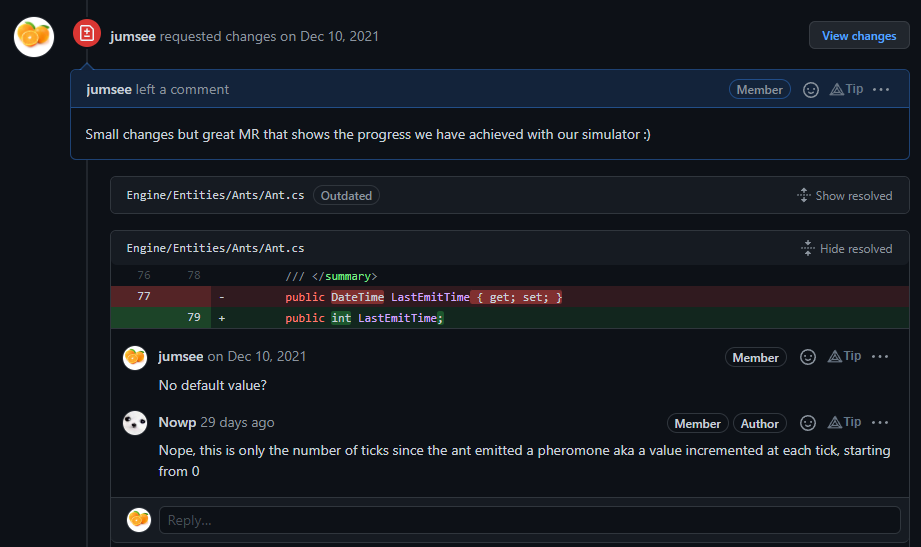
\includegraphics[scale=.5]{MergeRequest.png}
\caption{Exemple de commentaire sur un merge request pour l'ajout de la disparition des phéromones.}
\label{fig:MergeRequest}
\end{figure}

\paragraph{}
En plus des merge requests, GitHub nous permet de créer des \textit{issues}.
Ces \textit{issues} peuvent être considérés comme des tâches qu'il reste à faire. Au sein de GitHub, nous
pouvons à tout moment nous approprier une tâche afin d'indiquer qu'on a commencé à travailler dessus.

\paragraph{}
Ces issues apparaissent au sein du Kanban\footnote{Au sein de ce projet le Kanban était notre tableau de bord et nous permettait de suivre 
l'avancement et de savoir ce qu'il restait à faire. Plus d'informations : \url{https://en.wikipedia.org/wiki/Kanban_(development)}.}
intégré à GitHub. Nous avions deux Kanbans, un pour le côté Application et l'autre pour le moteur de simulation.

\begin{figure}[h]
\centering
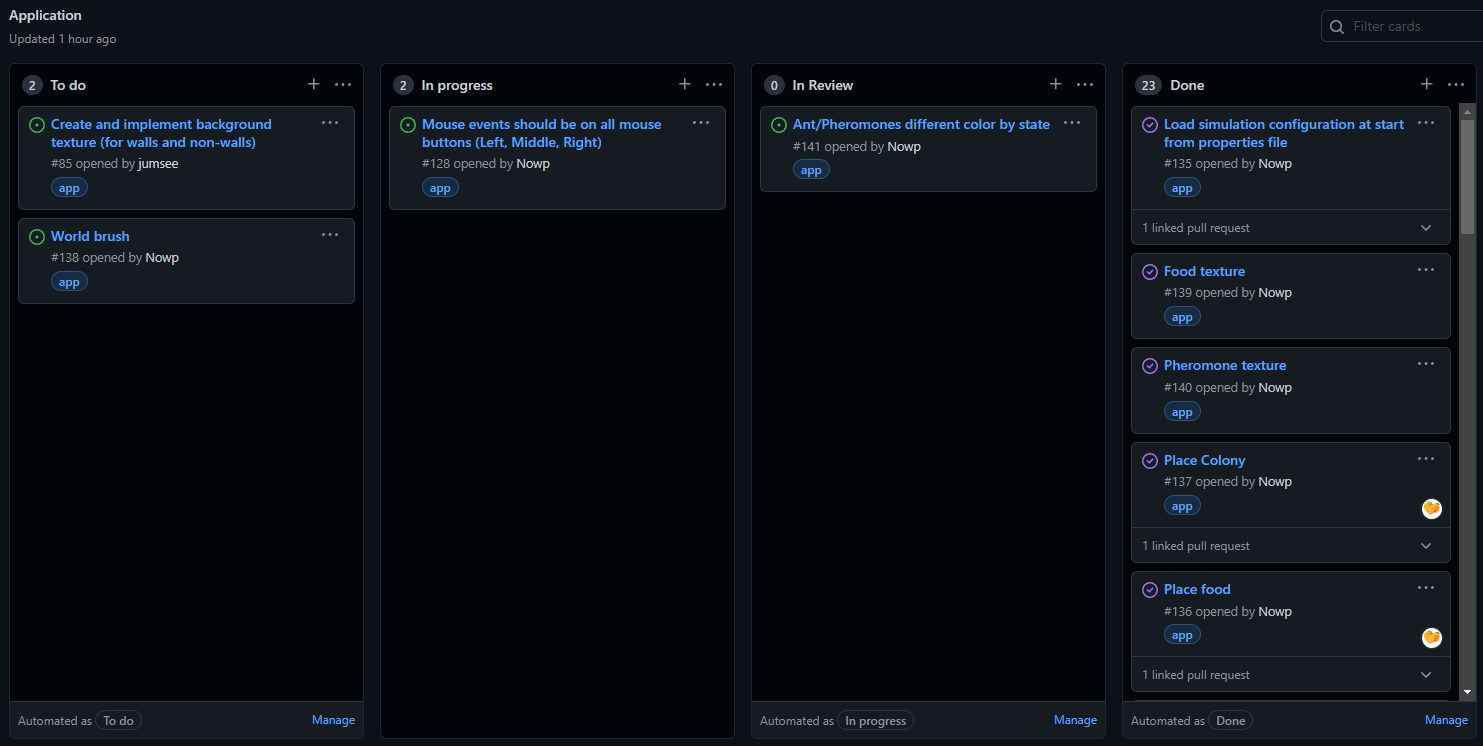
\includegraphics[scale=.4]{Kanban.png}
\caption{Exemple du tableau de bord côté Application. 
\\On voit les tâches qui sont en cours de développement et ceux qui sont prêts à être review.}
\label{fig:Kanban}
\end{figure}

\paragraph{}
Un autre élément que nous avons utilisé avec GitHub est la fonctionnalité d'intégration continue. En effet, nous avons configuré notre projet 
pour lancer tous les tests unitaires à chaque commit effectué sur une branche.
Cela nous a permis de repérer des erreurs dans notre code car nous n'avions pas le droit de merge une branche lorsque les tests n'étaient pas tous valides.

\subsection{Langage et Langue}

\paragraph{}
Le choix du langage de programmation à utiliser était une décision importante à prendre. Nous avons décidé de coder le projet en C\# car c'est un langage que nous
n'avons pas encore pu utiliser dans un gros projet. Nous étions au courant du fait que le C\# était très proche du Java et donc il n'y avait pas
d'inquiétudes sur notre capacité à l'apprendre. Le C\# reprend aussi les concepts de machine virtuelle qui existent en Java ce qui permettrait de build et lancer le projet
sur n'importe quel système d'exploitation grâce à .net. 
De plus, le C\# est un langage que nous avions pu utiliser lors de petit projets sur Unity mais jamais sur un gros projet comme celui-ci. 
A l'intérieur de C\# le standard de documentation utilisé est XMLdoc\footnote{Plus d'informations : \url{https://docs.microsoft.com/en-us/dotnet/csharp/language-reference/xmldoc/}.}.

\paragraph{}
Pour ce qui est de la langue dans laquelle nous avons codé, nous avons décidé de tout faire en Anglais pour que le code soit facilement
transmissible et exploitable par d'autres individus dans le monde.

\subsection{Librairie de Tests}

\paragraph{}
Il existe plusieurs librairie de test au sein de l'environnement dotnet. Les plus utilisés sont XUnit, NUnit et MSTest.
La bibliothèque que nous avons choisi d'utiliser est XUnit en raison du fait que Noé l'avait déjà utilisé au sein un autre projet.

\subsection{Framework d'affichage}

\paragraph{}
Au lancement du projet, nous avons dû réfléchir à quel framework utiliser pour faire l'affichage de la simulation.
Dans un premier temps, nous nous étions intéressé à Avalonia, un framework cross-platform qui est un successeur spirituel de WPF\footnote{WPF ou Windows Presentation Foundation est un framework permettant
de faire une interface graphique. Aujourd'hui il a beaucoup vieilli et est en train d'être remplacé par des frameworks plus modernes.}.
On s'est rendu compte qu'Avalonia n'était pas du tout ce qu'on recherchait comme il ne servait qu'à faire des interfaces graphiques et était très peu utilisable pour l'affichage de formes plus complexes.

\paragraph{}
Nous avons donc dû rechercher une solution alternative et c'est là que nous avons découvert MonoGame. 
MonoGame est un framework graphique open-source utilisé principalement pour des jeux comme son nom l'indique et qui est basé
sur le framework XNA (développé par Microsoft et abandonné depuis 2013). 
Après avoir consulté la documentation MonoGame nous avons pris la décision d'utiliser ce framework. Il nous a permis de simplifier les aspects tels que l'importation et l'utilisation de textures
et le dessin d'objets à l'écran.

\paragraph{}
En complément de MonoGame, l'ensemble des textures présent dans le projet ont été créé à la main par nous sur Piskel\footnote{Outil gratuit de dessin de PixelArt en-ligne. 
Plus d'informations : \url{https://www.piskelapp.com/}.}. 

\section{Moteur}

\subsection{Abstraction des Colliders}

\paragraph{}
Lorsque nous avons codé les colliders, nous nous sommes rendu compte que la manière initiale dont nous l'avions conçu
faisait qu'il y avait énormément de duplication de code et qu'il était difficilement maintenable.
La solution à cela était de déplacer les méthodes de collision dans une classe statique et ensuite chaque collider fait appel à la méthode qu'il a besoin dans la classe statique.



\section{Application}

\section{Tests}

\chapter{Résultats et perspectives}

\section{État des lieux}
\section{Apports}

\section{Évolutions possibles}


%--------------------------------------------------------------------------------
\chapter*{Conclusion}
\addcontentsline{toc}{chapter}{\numberline{}Conclusion}
\markboth{Conclusion}{}
 ultricies ut accumsan magna interdum. Nullam ut malesuada urna. Donec ut sem est. Curabitur ut neque elit. Sed aliquam sodales libero ut rutrum. Duis eu massa quam, rutrum posuere sapien. Suspendisse turpis nulla, eleifend ut faucibus consequat, laoreet varius tortor. Vestibulum accumsan sagittis hendrerit. Nunc tristique ligula quis ligula faucibus adipiscing. Aenean interdum, odio at volutpat interdum, justo nunc tristique elit, quis elementum nisi ante id arcu. Mauris commodo posuere cursus. Ut nec massa odio. Maecenas at eros arcu, quis rhoncus magna. Sed pellentesque dictum nulla nec pretium.

%--------------------------------------------------------------------------------
%exemple de bibliographie
\begin{thebibliography}{99}
\label{sec:biblio}
\bibitem{ref1}  détail bibliographique de la ref1
\bibitem{ref2}  détail bibliographique de la ref2
\bibitem{ref3}  détail bibliographique de la ref3
\bibitem{ref4}  détail bibliographique de la ref4
\bibitem{ref5}  détail bibliographique de la ref5
\end{thebibliography}


%--------------------------------------------------------------------------------
%si on donne des annexes :
\appendix
\addcontentsline{toc}{part}{\numberline{}Annexes}

%--------------------------------------------------------------------------------

\chapter{Liens utiles\label{sec:liens_utiles}}
Voici une petite liste d'url intéressantes au sujet de ce projet :

\begin{itemize}
\item {\url{https://github.com/PolyNoradrenalin/AntSimulator} Répertoire GitHub du projet}
\end{itemize}

%--------------------------------------------------------------------------------
%index : attention, le fichier dindex .ind doit avoir le même nom que le fichier .tex
%\printindex

%--------------------------------------------------------------------------------
%page du dos de couverture :

\resume{Integer lorem purus, rutrum quis lacinia in, egestas ut urna. Donec elementum mi id nisi blandit quis ultricies risus semper. Nulla congue tincidunt diam, id tincidunt mauris euismod nec. Nullam faucibus dapibus eros, at consequat odio rutrum quis. Curabitur nisl sem, suscipit in mattis eu, varius a mauris. Ut a augue ac augue fringilla egestas. Etiam non augue felis, in convallis nisi. Maecenas id urna ut justo tempor laoreet in eu ligula. Duis non erat vitae eros rhoncus rutrum sit amet at lorem. Ut tempor cursus ligula, eu bibendum ligula adipiscing eu. Fusce feugiat aliquam dolor, nec interdum nisl convallis vitae.}

\motcles{???, ????, ?????, ?????????, ??, ????}

\abstract{Integer lorem purus, rutrum quis lacinia in, egestas ut urna. Donec elementum mi id nisi blandit quis ultricies risus semper. Nulla congue tincidunt diam, id tincidunt mauris euismod nec. Nullam faucibus dapibus eros, at consequat odio rutrum quis. Curabitur nisl sem, suscipit in mattis eu, varius a mauris. Ut a augue ac augue fringilla egestas. Etiam non augue felis, in convallis nisi. Maecenas id urna ut justo tempor laoreet in eu ligula. Duis non erat vitae eros rhoncus rutrum sit amet at lorem. Ut tempor cursus ligula, eu bibendum ligula adipiscing eu. Fusce feugiat aliquam dolor, nec interdum nisl convallis vitae.}

\keywords{???, ????, ?????, ?????????, ??, ????}


\makedernierepage


\end{document}
%%FIN du fichier